% ****** Start of file apssamp.tex ******
%
%   This file is part of the APS files in the REVTeX 4.1 distribution.
%   Version 4.1r of REVTeX, August 2010
%
%   Copyright (c) 2009, 2010 The American Physical Society.
%
%   See the REVTeX 4 README file for restrictions and more information.
%
% TeX'ing this file requires that you have AMS-LaTeX 2.0 installed
% as well as the rest of the prerequisites for REVTeX 4.1
%
% See the REVTeX 4 README file
% It also requires running BibTeX. The commands are as follows:
%
%  1)  latex apssamp.tex
%  2)  bibtex apssamp
%  3)  latex apssamp.tex
%  4)  latex apssamp.tex
%
\documentclass[%
 reprint,
%superscriptaddress,
%groupedaddress,
%unsortedaddress,
%runinaddress,
%frontmatterverbose, 
%preprint,
%showpacs,preprintnumbers,
%nofootinbib,
%nobibnotes,
%bibnotes,
 amsmath,amssymb,
 aps,
%pra,
%prb,
%rmp,
%prstab,
%prstper,
%floatfix,
]{revtex4-1}

\usepackage{graphicx}% Include figure files
\usepackage{dcolumn}% Align table columns on decimal point
\usepackage{bm}% bold math
%\usepackage{hyperref}% add hypertext capabilities
%\usepackage[mathlines]{lineno}% Enable numbering of text and display math
%\linenumbers\relax % Commence numbering lines

%\usepackage[showframe,%Uncomment any one of the following lines to test 
%%scale=0.7, marginratio={1:1, 2:3}, ignoreall,% default settings
%%text={7in,10in},centering,
%%margin=1.5in,
%%total={6.5in,8.75in}, top=1.2in, left=0.9in, includefoot,
%%height=10in,a5paper,hmargin={3cm,0.8in},
%]{geometry}

\begin{document}

\preprint{APS/123-QED}

\title{A New Novel Trap For Neutral Atoms}% Force line breaks with \\
\thanks{A footnote to the article title}%

\author{D. Lobser}
 \altaffiliation[Also at ]{Physics Department, XYZ University.}%Lines break automatically or can be forced with \\
%\author{Second Author}%
 %\email{Second.Author@institution.edu}
%\affiliation{%
 %Authors' institution and/or address\\
 %This line break forced with \textbackslash\textbackslash
%}%

%\collaboration{MUSO Collaboration}%\noaffiliation

%\author{Charlie Author}
 %\homepage{http://www.Second.institution.edu/~Charlie.Author}
%\affiliation{
 %Second institution and/or address\\
 %This line break forced% with \\
%}%
%\affiliation{
 %Third institution, the second for Charlie Author
%}%
%\author{Delta Author}
%\affiliation{%
 %Authors' institution and/or address\\
 %This line break forced with \textbackslash\textbackslash
%}%
%
%\collaboration{CLEO Collaboration}%\noaffiliation

\date{\today}% It is always \today, today,
             %  but any date may be explicitly specified

\begin{abstract}
A modification to the standard Time-averaged Orbiting Potential (TOP) trap that allows for very isotropic potentials.
\begin{description}
\item[Usage]
Secondary publications and information retrieval purposes.
\item[PACS numbers]
May be entered using the \verb+\pacs{#1}+ command.
\item[Structure]
You may use the \texttt{description} environment to structure your abstract;
use the optional argument of the \verb+\item+ command to give the category of each item. 
\end{description}
\end{abstract}

\pacs{Valid PACS appear here}% PACS, the Physics and Astronomy
                             % Classification Scheme.
%\keywords{Suggested keywords}%Use showkeys class option if keyword
                              %display desired
\maketitle

%\tableofcontents

\section{\label{sec:level1} Introduction}
%The Time-averaged Orbiting Potential (TOP) trap was developed in 1993 for the creation of the first Bose-Einstein condensate (BEC). Since the first realization of BEC, numerous magnetic traps have been developed which displace the magnetic zero away from the trap center. The TOP trap is able to generate the extremely cylindrical potentials necessary for vortex experiments where the roundness of the trap was critical for maintaining the large angular momentum of the condensate. In the strong field limit, the axial and radial spring constants have a ratio of $\sqrt{8}$. By reducing the strength of the quadrupole field, gravitational effects cause this ratio to decrease, allowing for a spherical potential. However, construction asymmetries can only be shimmed out in the xy plane preventing full control over the ellipsoidal shape of the potential. Through the addition of a third oscillating field, we gain control over all of the elliptic cross terms allowing for an extremely isotropic potential.

%Over a century ago, Boltzmann derived his famous H-theorem to describe entropy using mechanical arguments. His theories met with a vicious opposition because the time reversal symmetry inherent to mechanical systems conflicted with the irreversible nature of entropy. This was said to have aggravated his bouts of depression and ultimately led to his suicide in 1906. In a series of heated articles, Boltzmann did acknowledge that certain exotic cases exist that could lead to bizarre collective behavior but dismissed them as irrelevant to the description of naturally occurring systems. One case in particular was that a gas confined to a perfectly spherical harmonic potential wouldn't necessarily reach equilibrium. Namely, the monopole motion of the gas is \textit{undamped}. Experimental study of this particular phenomenon has so far been prevented by the difficulty in generating a sufficiently isotropic harmonic potential. 

The mechanical basis for Boltzmann\'s derivation of the H-theorem incited a series of attacks against his theories.
In response to an article concerning the conflict between the time reversal symmetry inherent to mechanical systems and the irreversible nature of entropy, Boltzmann explicitly showed a number of situations where the initial conditions of a system could be artifically constructed to produce bizarre collective behavior.
Among these specific cases was the fact that a gas might never reach equilibrium in a perfectly isotropic harmonic potential, and in particular the monopole mode of a gas would be \textit{undamped}~\cite{Cercignani1988}.
Experimental study of this particular phenomenon has so far been prevented by the difficulty in generating a sufficiently isotropic harmonic potential. 


%This opposition to Boltzmann's views was said to have aggravated his bouts of depression and ultimately led to his suicide in 1906. 

%Over a century ago, Boltzmann developed his transport equation to describe how gaseous systems reach equilibrium, which ultimately led to a model of the 2nd law of thermodynamics known as the H-theorem. His theories met with a vicious opposition because they derived from mechanical arguments and the inherent time reversal symmetry of mechanical systems conflicted with the irreversible nature of entropy. This opposition to Boltzmann's views was said to have aggravated his bouts of depression and in 1906 he committed suicide. Boltzmann never wavered in his views and adamantly defended the validity of his approach. Despite the arguments against his theories, he explicitly showed that a gas confined in a spherical harmonic potential won't necessarily reach equilibrium. In particular, the monopole, or ``breathe'' mode, of a gas is expected to be completely \textit{undamped}. This effect has never been experimentally verified because of the difficulty in creating a spherical harmonic potential. We have developed a new magnetic trap which is capable of generating a potential which is spherical to within 99.9\%

The theoretical issues which fueled the debate stem from the Boltzmann equation. For a phase space distribution,  $f \equiv f\left(\mathbf{r},\mathbf{p},t\right)$, the Boltzmann equation in its simplest form is
\begin{equation}
\frac{df}{dt} = I_{coll}\left[f\right],
\end{equation}
where $I_{coll}\left[f\right]$ is a collision function, referred to as the \textit{collision integral}. Essentially, the Boltzmann states that the phase space distribution of a gas approaches equilibrium at a rate proportional to the frequency of collisions. At equilibrium, the distribution becomes stationary and the collision integral vanishes. Expanding the derivative and including the explicit definition of  $I_{coll}\left[f\right]$ leads to the more standard form of the Boltzmann equation

%where $f \equiv f\left(\mathbf{r},\mathbf{p},t\right)$ is the probability density of finding a particle at a given phase space coordinate, and $I_{coll}\left[f\right]$ is a collision function. Essentially, the Boltzmann equation states that the distribution of particles in a gas approaches equilibrium at a rate proportional to the frequency of collisions. When equilibrium is reached, the distribution becomes stationary and the collisional contribution vanishes. Expanding the derivative and including the explicit definition of $I_{coll}\left[f\right]$, the Boltzmann equation takes on the more standard form

%In a confining potential, the distribution takes on a spatial dependence and $f = f\left(\mathbf{r},\mathbf{p},t\right)$. Expanding the derivative and including the explicit definition of $I_{coll}\left[f\right]$, the Boltzmann equation takes on the more standard form
%\begin{eqnarray}
%\frac{\partial f}{\partial t} + \mathbf{v}_1\cdot\nabla_\mathbf{r}f+\frac{\mathbf{F}}{m}\cdot\nabla_{\mathbf{v}_1}f = \frac{\sigma_0}{4\pi} \int d^2\Omega d^3\mathbf{v}_2\left|\mathbf{v}_2-\mathbf{v}_1\right|\left(f_1'f_2'-f_1f_2\right)~~~~~~~~~~~~~~~~~ \nonumber\\
% \times \delta\left(\mathbf{p}_1+\mathbf{p}_2 - \mathbf{p}_1'-\mathbf{p}_2'\right)   \delta\left(p_1^2+p_2^2 - p_1'^2-p_2'^2\right)
%\end{eqnarray}
%Typically, energy and momentum conservation is implicitly assumed and the delta functions are omitted in the standard literature.
\begin{eqnarray}
\frac{\partial f}{\partial t}&+&\mathbf{v}_1\cdot\nabla_\mathbf{r}f+\frac{\mathbf{F}}{m}\cdot\nabla_{\mathbf{v}_1}f = \label{eq:boltzmann}\\
& &\frac{\sigma_0}{4\pi} \int d^2\Omega d^3\mathbf{v}_2\left|\mathbf{v}_2-\mathbf{v}_1\right|\left(f(\mathbf{v}_1')f(\mathbf{v}_2')-f(\mathbf{v}_1)f(\mathbf{v}_2)\right)\nonumber
\end{eqnarray}
where $\sigma_0$ is the collision cross section. Energy and momentum conservation are implicitly assumed, but could easily be included in the collision integral using a delta function. The other major assumption is that the atoms can be treated as hard spheres, but this approximation is valid for \textit{s}-wave collisions when mean field effects are negligible and the cloud is non-degenerate. %As the cloud becomes highly degenerate, Bose enhancement terms must be taken into account and Eq.~\ref{eq:boltzmann} becomes
%\begin{equation}
%\frac{\partial f}{\partial t} + \mathbf{v}_1\cdot\nabla_\mathbf{r}f+\frac{\mathbf{F}}{m}\cdot\nabla_{\mathbf{v}_1}f =\frac{\sigma_0}{4\pi}\int d^2\Omega d^3\mathbf{v}_2\left|\mathbf{v}_2-\mathbf{v}_1\right|\left(f_1'f_2'(1+h^3f_1)(1+h^3f_2)-f_1f_2(1+h^3f_1')(1+h^3f_2')\right).
%\label{eq:boltzmann}
%\end{equation}
%The distribution functions in the Bose enhancement terms are scaled by $h^3$ where $h$ is Planck's constant, and for a thermal cloud the enhancement terms are approximately unity.

Distributions of the form
\begin{equation}
\log f = \alpha + \mathbf{\beta}\cdot\mathbf{v}+\gamma v^2
\label{eq:collisioninvariant}
\end{equation}
cause the collision integral to vanish due to conservation of energy and momentum and are referred to as \textit{collisionally invariant}.
These distributions, generally called local equilibrium distributions, do not necessarily satisfy Eq.~\ref{eq:boltzmann} and constraints must be placed on $\alpha$, $\beta$, and $\gamma$.
For a sufficiently general outside potential, these constants can be constrained to produce an equilibrium distribution equivalent to Maxwell-Boltzmann~\cite{UhlenbeckFord}.
For certain special potentials, collisionally invariant distributions exist that satisfy Eq.~\ref{eq:boltzmann}.
For an isotropic harmonic potential, the solution is an equilibrium distribution undergoing temperature oscillations where the spatial distribution varies identically such that the distribution satisfies the equilibrium constraint at each instant in time.
The undamped nature of the monopole mode is found by computing the evolution of the square radius and can be derived in various ways~\cite{Guery-Odelin1999}, but we find that it can easily be elucidated by the two particle case.


%Persistence of monopole oscillations can be described in various ways\cite{Guery-Odelin1999}
 %but can be elucidated by the two particle case. 

Spherical symmetry simplifies the problem, which can be treated as analogously one dimensional, and the radial motion of a single particle of mass $m$, energy $E$ and angular momentum $L$ is governed by the effective potential
\begin{equation}
V_e = \frac{L^2}{2mr^2}+\frac{1}{2}m\omega^2r^2.
\end{equation}
The radial force,
\begin{equation}
m\frac{d^2r}{dt^2} = -\frac{d}{dr}V_e,
\label{eq:radialforce}
\end{equation}
can be combined with the kinetic energy,
\begin{equation}
\frac{1}{2}m\left(\frac{dr}{dt}\right)^2 = E-V_e,
\end{equation}
by integrating Eq.~\ref{eq:radialforce}. This yields
\begin{equation}
\frac{d^2}{dt^2}r^2 = -\Omega^2\left(r^2-r_0^2\right),
\end{equation}
where $\Omega\equiv2\omega$ and $r_0^2=E/(m\omega^2)$, so that the square radius undergoes sinusoidal oscillations around its mean value $r_0^2$ at a frequency of $2\omega$. If there are 2 particles, 1 and 2, each with individual values of E, L and $r^2$, each particle will oscillate at $2\omega$ and taking the linear combination of their respective differential equations yields
\begin{equation}
\frac{d^2}{dt^2}r_t^2 = -\Omega^2\left(r_t^2-r_{0t}^2\right)
\label{eq:monopolecomb}
\end{equation}
so their combined square radius, $r_t^2 = r_1^2+r_2^2$, oscillates around its mean value, $r_{0t}^2 = (E_1+E_2)/(m\omega^2)$. The magnitude of the monopole motion depends on the magnitude and relative phase of the individual particle trajectories. These individual quantities will abruptly change in the event of a collision. Assuming the collisions are local, $r_1$, $r_2$, and thus $r_t^2$ will not change from the instant before to the instant after the collision. Similarly, momentum and energy conservation imply that $\frac{d}{dt}r_t^2$ and $r_{0t}^2$ are unchanged by the collision. These three continuities imply that the parameters and boundary conditions of Eq.~\ref{eq:monopolecomb} are matched directly before and after a collision. This ensures that neither the magnitude or phase of the oscillation will change as the result of a pairwise collision. Generalizing to N atoms, so that
\begin{equation}
r_t^2 = \sum_{i=1}^Nr_i^2
\end{equation}
and
\begin{equation}
r_{0t}^2 = \frac{1}{m\omega^2}\sum_{i=1}^NE_i,
\end{equation}
one can see that the monopole mode is left unperturbed--and in particular \textit{undamped}--by local, pairwise, momentum- and energy-conserving collisions.
 
For the quadrupole mode, the damping rate is given by
\begin{equation}
\Gamma_Q = \frac{1}{5} n\left(0\right)\sigma \bar{v},
\label{eq:quaddamprate}
\end{equation} 
where $n_{cl}\left(0\right)$ is the peak atomic density, $\sigma$ is the scattering cross section given by $8\pi a^2$, and $\bar{v}$ is the average thermal velocity. 



Experimentally, we evaporatively cool $^{87}$Rb atoms in a new magnetic trap capable of generating an isotropic harmonic potential with trap frequencies that differ by less than 0.1\%. Degeneracy effects are minimized by keeping cloud temperatures well above $T_c$. Monopole mode damping rates are compared against quadrupole mode damping rates, which are sufficiently fast and linearly dependent on collision frequency. We selectively drive monopole (quadrupole) motion by (a)symmetrically modulating the strength of the confinement about its mean value. The cloud is then allowed to propagate freely in the spherical trap before it is non-destructively imaged using phase contrast microscopy. Six images are taken of each cloud along two orthogonal axes with an interval of 17 ms in order to sample roughly 1.5 oscillation periods. Widths of the cloud along each dimension, $\sigma_i$, are determined from Gaussian surface fits of individual images and converted to monopole and quadrupole amplitudes through the following relations
\begin{equation}
A_M^i = \frac{\sigma_{xi}^2+\sigma_{yi}^2+\sigma_{zi}^2}{\langle \sigma_x^2+\sigma_y^2+\sigma_z^2\rangle}-1
\end{equation}
\begin{equation}
A_Q^i = \frac{2\sigma_{zi}^2-\sigma_{xi}^2+\sigma_{yi}^2}{\langle 2\sigma_z^2-\sigma_x^2+\sigma_y^2\rangle}-1
\end{equation}
where $i$ indicates the individual image and the average is taken over all images for a single run of the experiment.
Analysis is simplified by fitting the oscillation obtained from each experimental cycle with a fixed frequency sine wave, from which the relative oscillation amplitude is extracted, as indicated by the solid lines in Fig.~\ref{fig:quadbreathe}.

\begin{figure}[htb]

    \begin{center}
    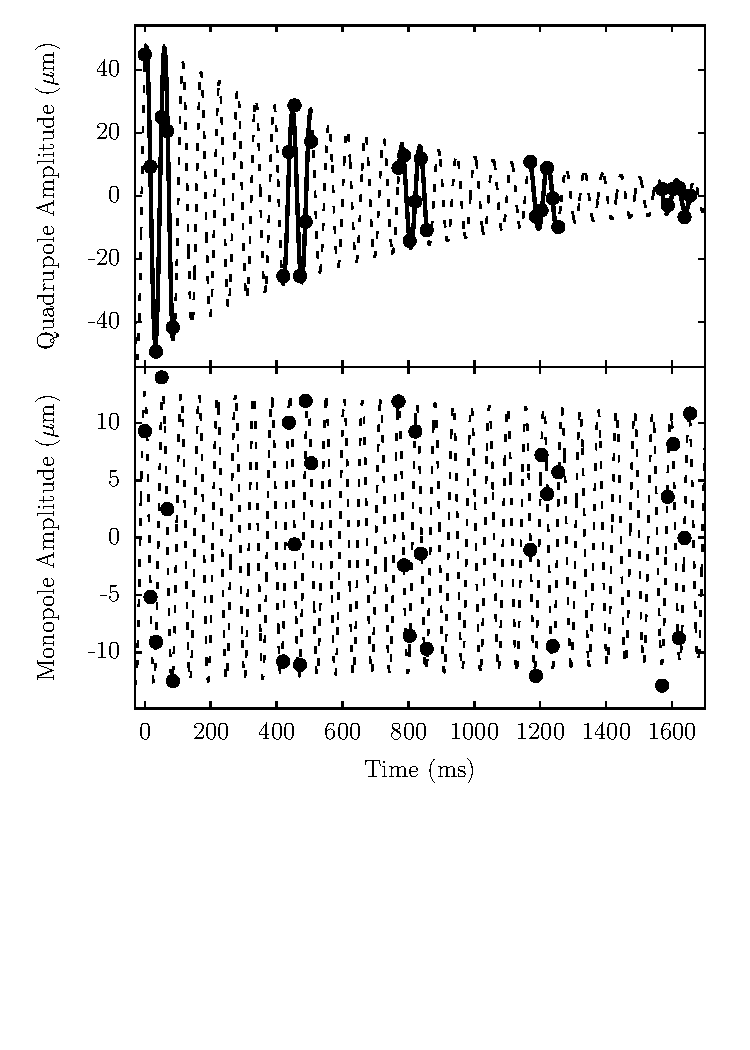
\includegraphics[width=80mm]{./figs/725QuadMonoStackedSHORT7.pdf}
    \end{center}
    \caption[damhere]{
        Sample data for a driven quadrupole mode and monopole mode in a spherical trap with $\vert f_z-f_r\vert/f_z < 0.002$.
        Black lines on the quadrupole data indicate a typical fitting procedure where individual periods taken in a single run are fit with an undamped sine wave to extract the amplitude.
    }
    \label{fig:quadbreathe}
\end{figure}

One sees the suppressed damping of the monopole mode from the sample data in Fig.~\ref{fig:quadbreathe}. From Eq.~\ref{eq:boltzmann}, the damping rate is found to be linearly proportional to the collision rate. 
%For the quadrupole mode, the damping rate is given by
%\begin{equation}
%\Gamma_Q = \frac{1}{5} n_{cl}\left(0\right)\sigma \bar{v},
%\label{eq:quaddamprate}
%\end{equation} 
%where $n_{cl}\left(0\right)$ is the peak atomic density, $\sigma$ is the scattering cross section given by $8\pi a^2$, and $\bar{v}$ is the average thermal velocity. 
By varying the evaporation parameters, we can tune the collision rate of of the sample and alternately drive quadrupole or monopole modes.
A direct comparison of quadrupole and monopole damping rates is shown in Fig.~\ref{fig:qbdamp}, where $\vert f_z-f_r\vert/f_z < 0.003$.
While the linear dependence on quadrupole damping rate is in good agreement with Eq.~\ref{eq:quaddamprate}, the monopole damping rate appears to be independent of collision rate.
\begin{figure}[htbl!]
    \begin{center}
    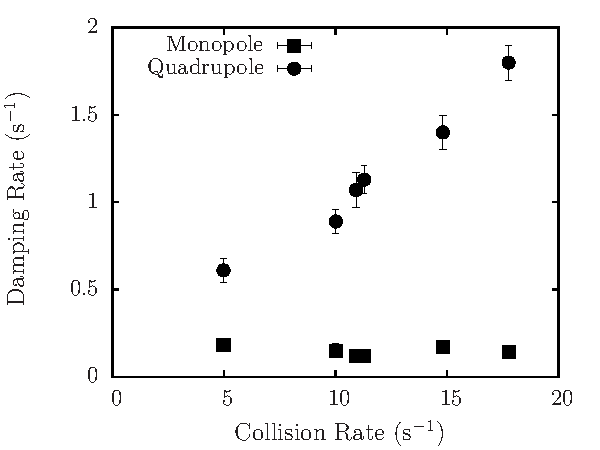
\includegraphics[width=80mm]{./figs/QuadBreathevsCollf3.pdf}
    \end{center}
    \caption[qbdamp]{
        Monopole and quadrupole damping rates as a function of interatomic collision rate. Each set was taken in very spherical traps where $\vert f_z-f_r\vert/f_z < 0.003$.
    }
    \label{fig:qbdamp}
\end{figure}

The average monopole damping rate is small, but still finite, with a mean value of $\Gamma_M = 0.14(3)$. This nonzero damping could be potentially due to small anisotropies in the trapping potential. With no collisions present, oscillations along the principal axes of the trap are fully decoupled and monopole- or quadrupole-like oscillations are totally undamped. If the principal trap frequencies differ such that $\omega_1=\omega_2\neq\omega_3$, dephasing occurs between oscillations along different principal axes and oscillations between monopole-like motion and purely quadrupole-like motion occur with a period given by
\begin{equation}
T_{MQ} = \frac{\pi}{\vert\omega_{1,2}-\omega_3\vert}.
\end{equation}
With collisions present, monopole-quadrupole oscillations lead to damping when the quadrupole motion is nonzero. This effect can be seen when $T_{MQ} < 1/\Gamma_Q$.


%The system becomes integrable and the energy in the monopole mode is a conserved quantity.



  

%\begin{figure}[htb]

    %\begin{center}
    %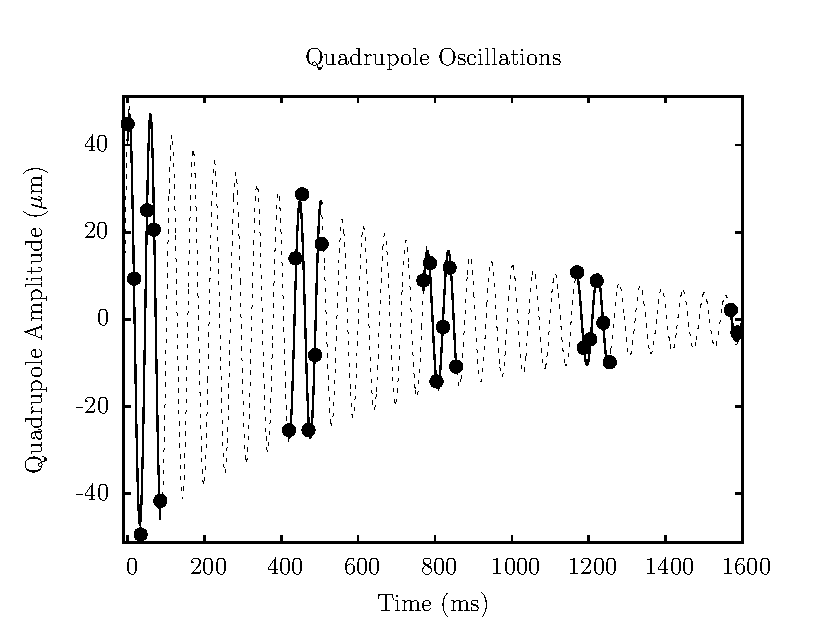
\includegraphics[width=40mm]{./figs/725QuadDecay.pdf}
    %%${}^{}$ 
    %%${}^{}$ 
    %%${}^{}$
    %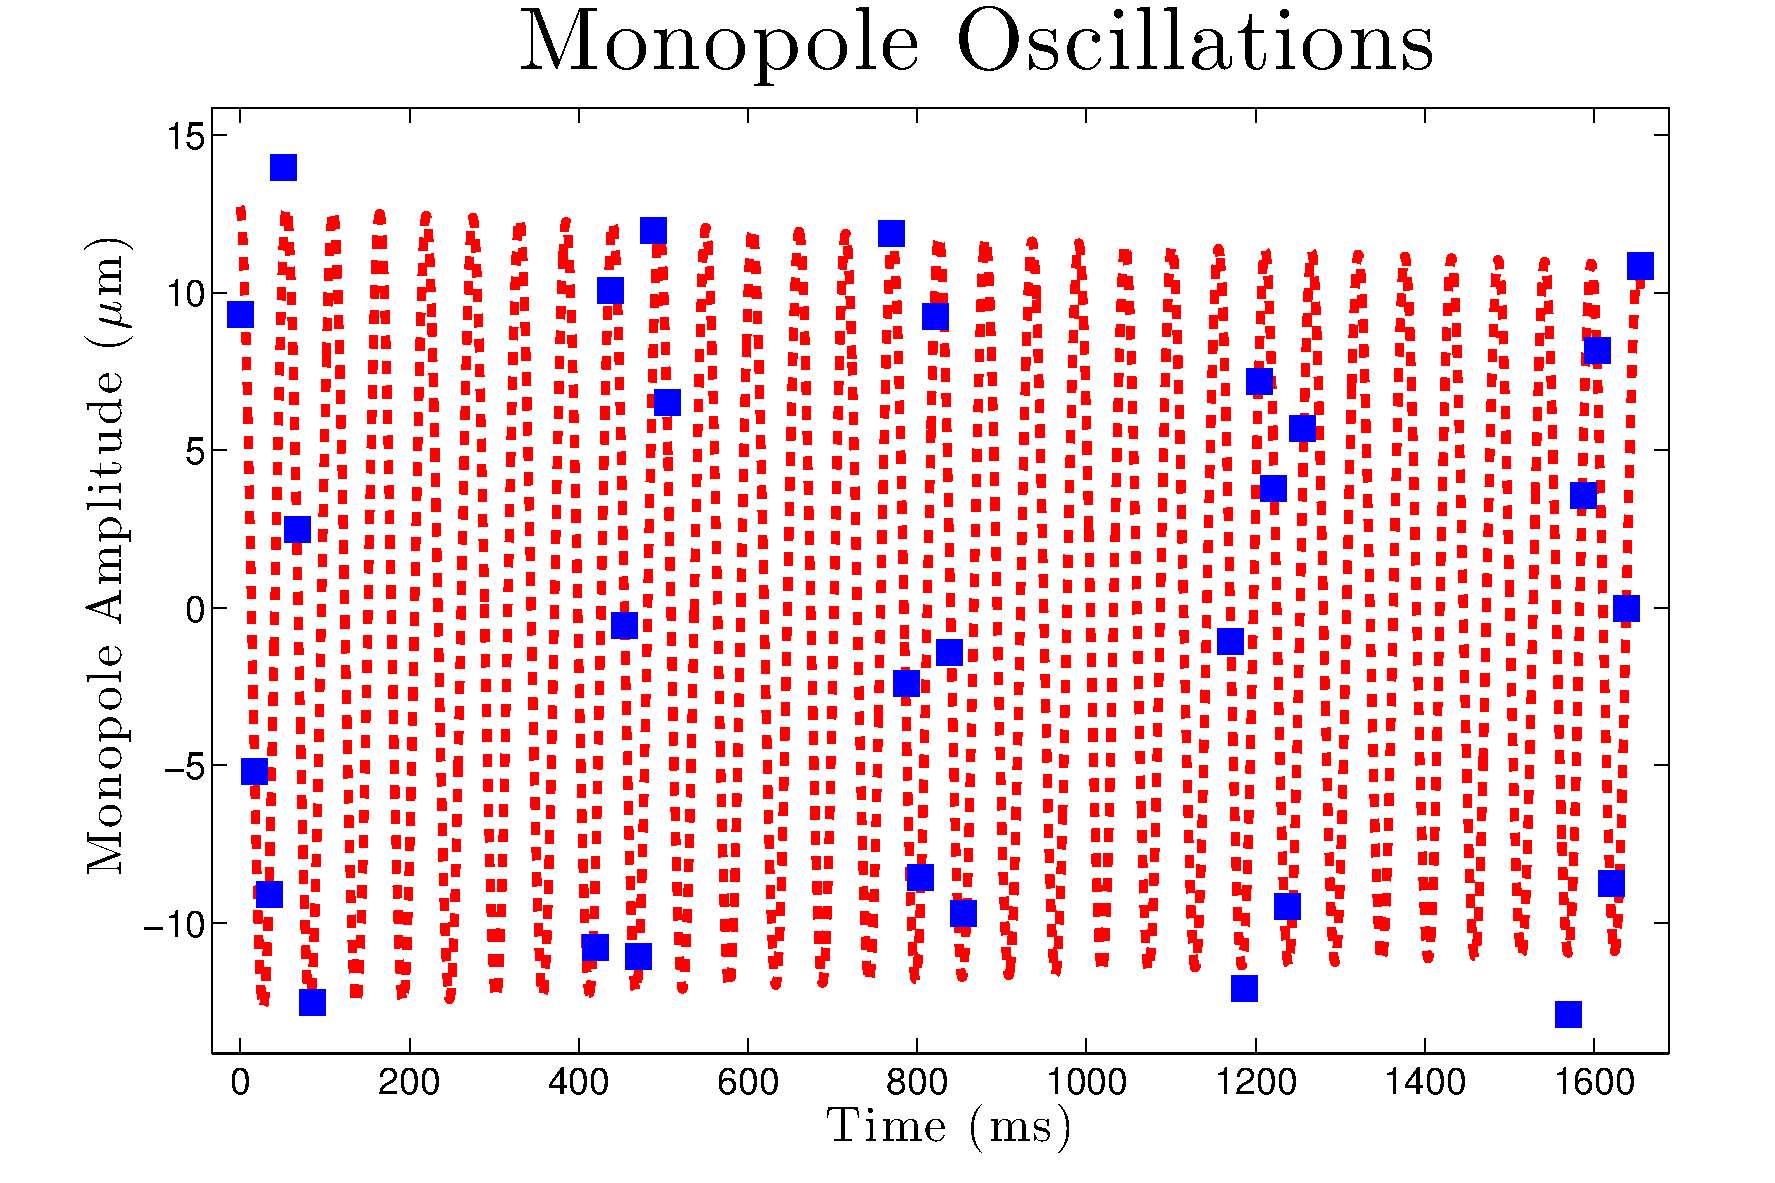
\includegraphics[width=40mm]{./figs/BreatheDecf56t106Short_v2.pdf}
    %\end{center}
    %\caption[Cutting up a triangular pyramid]{
        %Sample data for a driven quadrupole mode and monopole mode in a spherical trap.
        %Black lines on the quadrupole data indicate a typical fitting procedure where individual periods taken in a single run are fit with an undamped sine wave to extract the amplitude.
    %}
    %\label{pyramid}
%\end{figure}

%\begin{figure}[htb]
%
    %\begin{center}
    %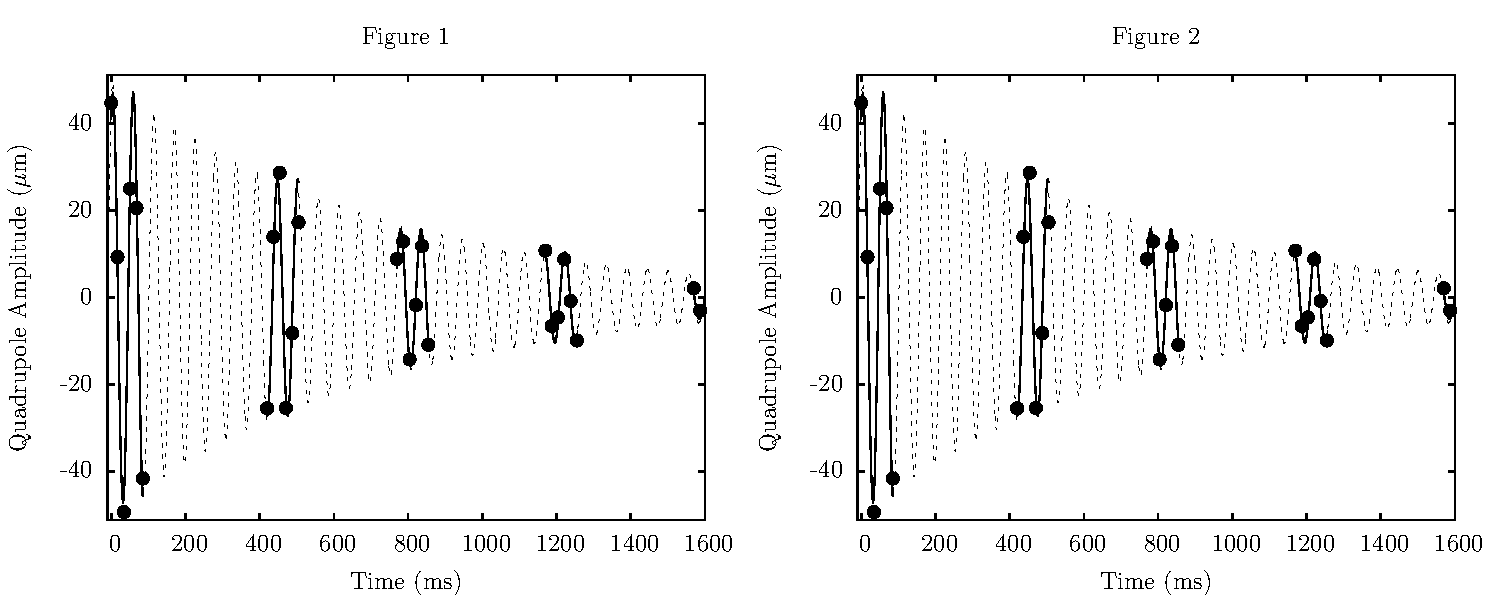
\includegraphics[width=80mm]{./figs/plottmp.pdf}
    %\end{center}
    %\caption[damhere]{
        %Sample data for a driven quadrupole mode and monopole mode in a spherical trap.
        %Black lines on the quadrupole data indicate a typical fitting procedure where individual periods taken in a single run are fit with an undamped sine wave to extract the amplitude.
    %}
%\end{figure}



%\begin{figure}[htb]
%
    %\begin{center}
    %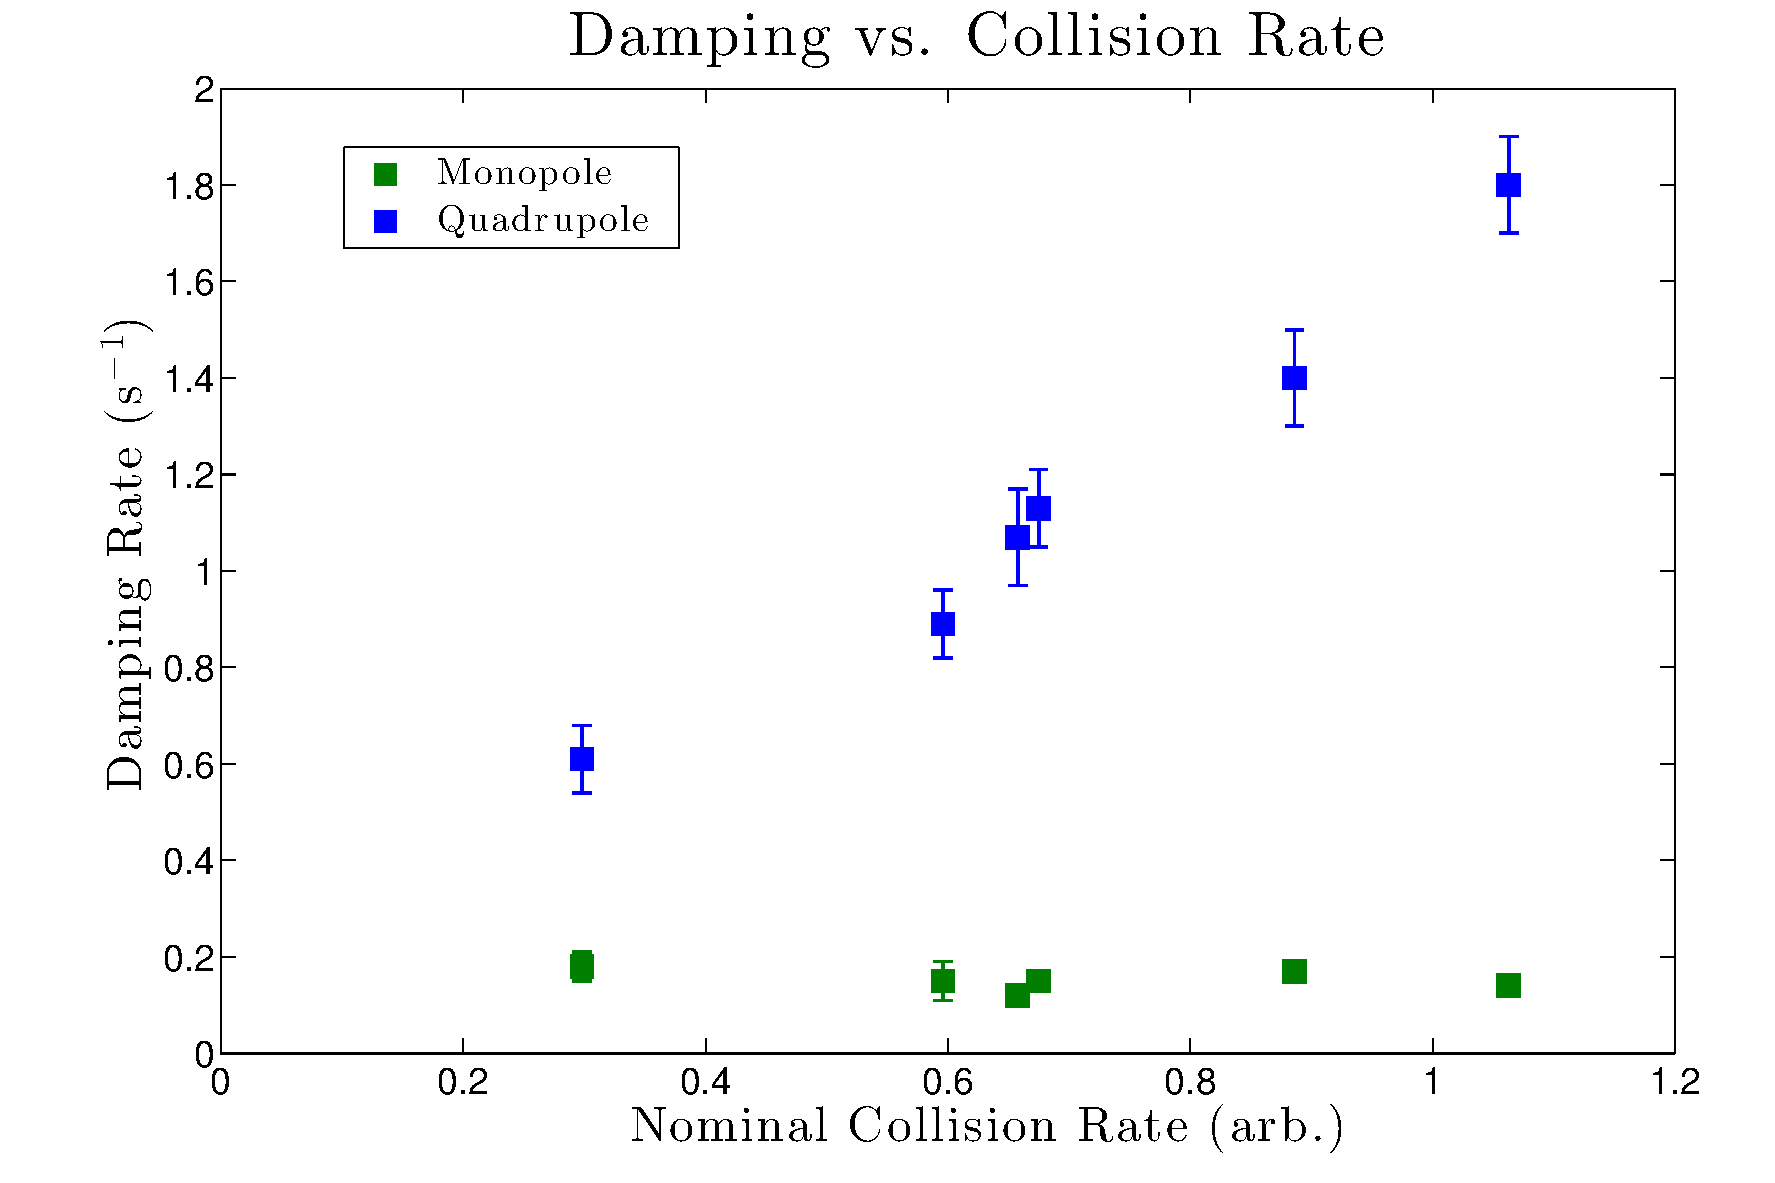
\includegraphics[width=80mm]{./figs/DampingvsCollRateSpherical_v2.pdf}
    %\end{center}
    %\caption[dampsphere]{
        %Sample data for a driven quadrupole mode and monopole mode in a spherical trap.
        %Black lines on the quadrupole data indicate a typical fitting procedure where individual periods taken in a single run are fit with an undamped sine wave to extract the amplitude.
    %}
%\end{figure}



\bibliography{ThermalBreathe2}% Produces the bibliography via BibTeX.

\end{document}
%
% ****** End of file apssamp.tex ******
